\chapter{Übersicht über elektronische Anhänge}

\begin{easylist}[itemize]
	& Bachelorarbeit in elektronischer Form
	& Bitstreams
	&& plasma\_soc.rbf
	& dts
	&& socfpga\_cyclone5\_de1\_soc.dtb
	&& socfpga\_cyclone5\_de1\_soc.dts
	&& socfpga\_cyclone5.dtsi
	&& socfpga.dtsi
	&& skeleton.dtsi
	& Plasma-SoC - Quelltexte
	&& proj - Vivado und Quartus Projektdateien
	&& rtl - Hardwarebeschreibung
	&& sw - Software
	&& tb - Testbenches
	&& dependencies 
	&&& KebabOS - Firmware-Quellcode
	&&& PlasmaConvert - ELF-Converter
	& Referenzen
	& Webquellen
	& README.md
	& linux-socfpga-socfpga-4.9.78-ltsi.zip
	&& Linux-Kernel-Quelltexte 4.9.78-ltsi
	&&& Als ZIP mitgeliefert, da auf dem MacOS das Dateisystem nicht Case-Sensitiv ist. 
	&& ubuntu-4.9.78.img.gz - modifiziertes Linux-Systemabbild
	&&&  Komprimiertes Image, zum direkten Beschreiben eines Gerätes bitte \texttt{gunzip -c ubuntu-4.9.78.img.gz | pv | sudo dd of=/dev/sdf bs=1M} ausführen
\end{easylist}
%\textsl{}
%
%\chapter{Serielle Verbindung}
%
%Die serielle Verbindung wird mit folgenden Parametern aufgebaut: 
%\begin{easylist}[itemize]
%	& Übertragungsgeschwindigkeit: 115200 Baud
%	& Datenbits: 8
%	& Stoppbits: 1
%	& Parität: keine
%	& Datenflusssteuerung: keine
%\end{easylist}
%
%Eine mögliche Konfiguration für Putty ist in \cref{fig:putty} dargestellt. Sobald die Verbindung erfolgreich aufgebaut wird, sollte der Terminal wie auf \cref{fig:putty_serial_connected} aussehen. 
%
%\begin{figure}[!htbp]
%	\centering
%	\begin{subfigure}{.5\textwidth}
%		\centering
%		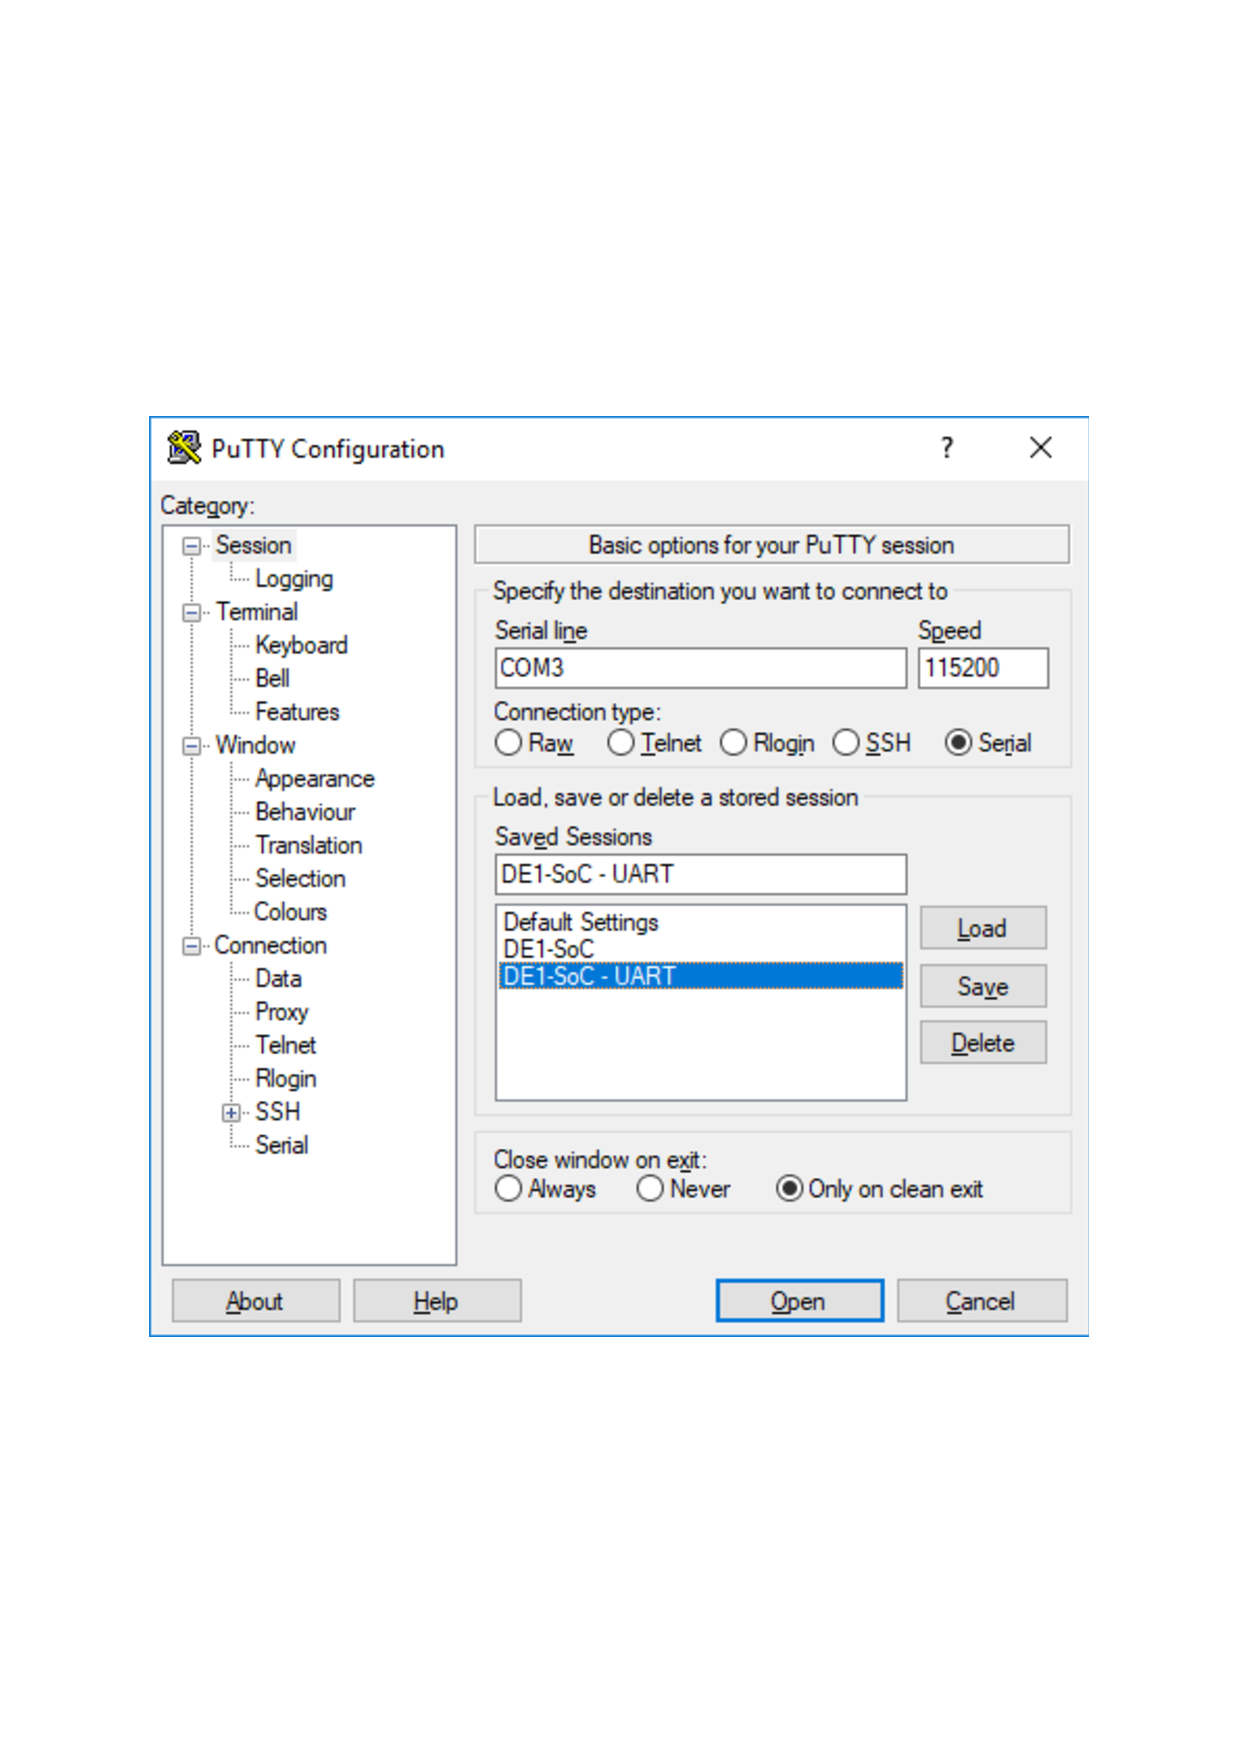
\includegraphics[width=0.9\linewidth]{images/putty_serial}
%		\caption{Grundeinstellungen}
%		\label{fig:putty_serial}
%	\end{subfigure}%
%	\begin{subfigure}{.5\textwidth}
%		\centering
%		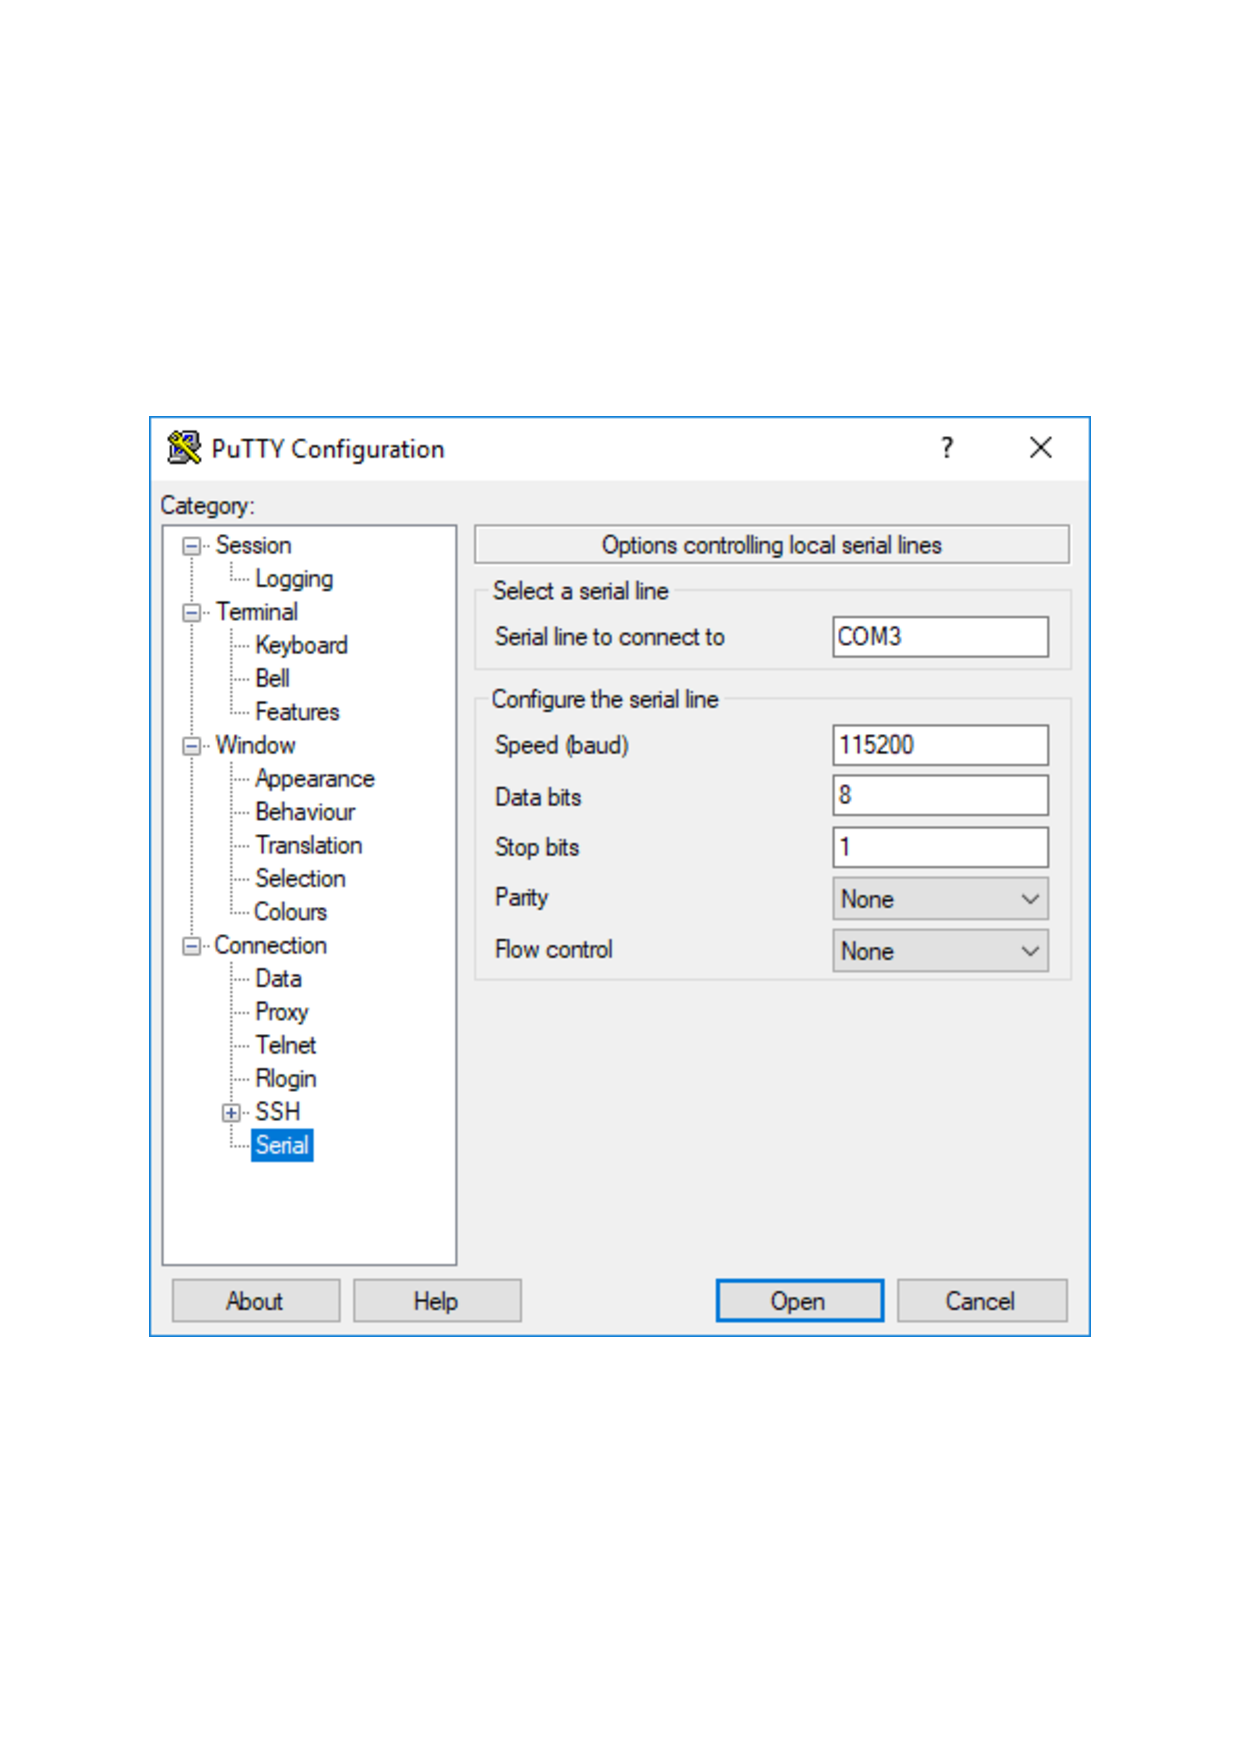
\includegraphics[width=0.9\linewidth]{images/putty_serial_params}
%		\caption{Erweiterte Einstellungen}
%		\label{fig:putty_serial_params}
%	\end{subfigure}
%	\caption{Putty-Konfiguration}
%	\label{fig:putty}
%\end{figure}
%
%\begin{figure}[!htbp]
%	\centering
%	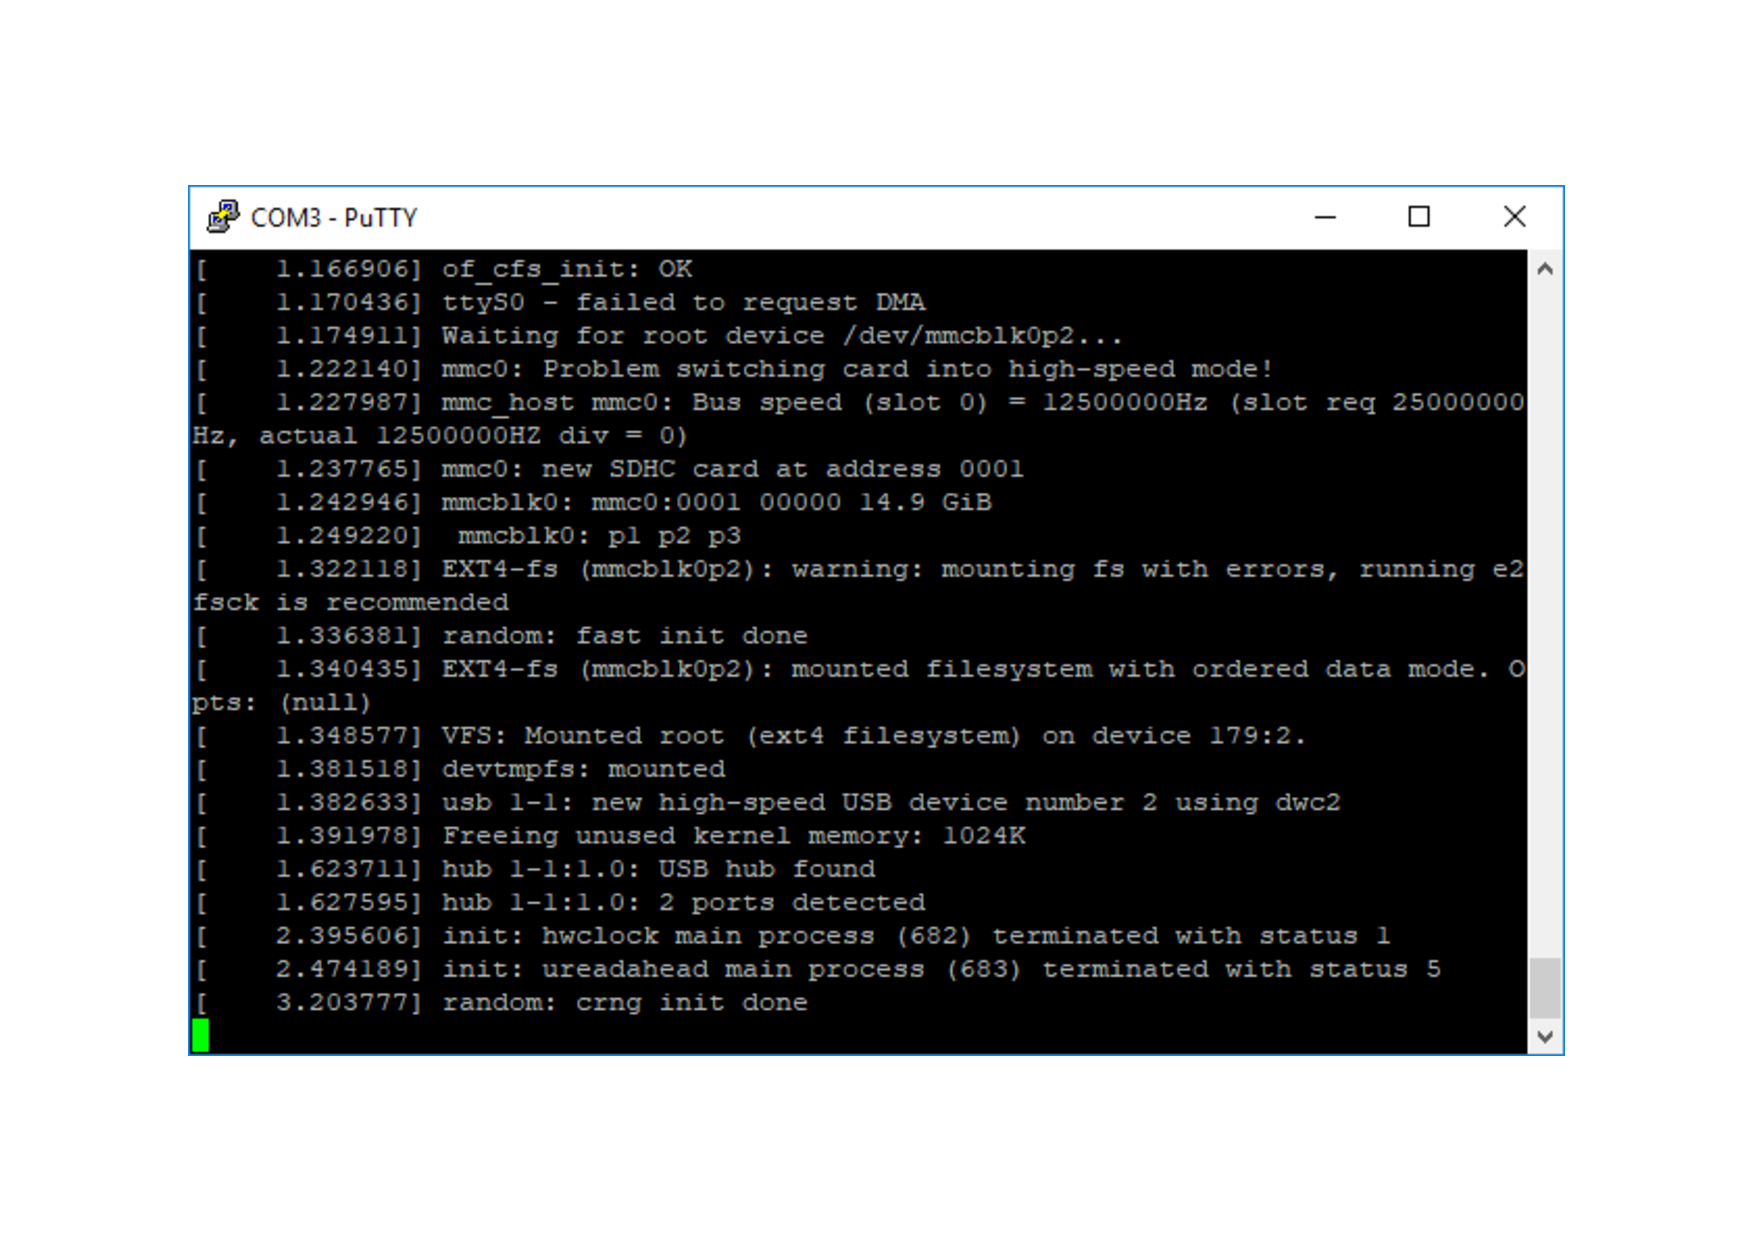
\includegraphics[width=1\linewidth]{images/putty_serial_connected}
%	\caption{Erfolgreich aufgebaute serielle Verbindung}
%	\label{fig:putty_serial_connected}
%\end{figure}
%
%
%\chapter{VNC Verbindung}
%
%Auf dem 
%%\begin{figure}[!htbp]
%%	\centering
%%	\begin{subfigure}{.5\textwidth}
%%		\centering¬
%%		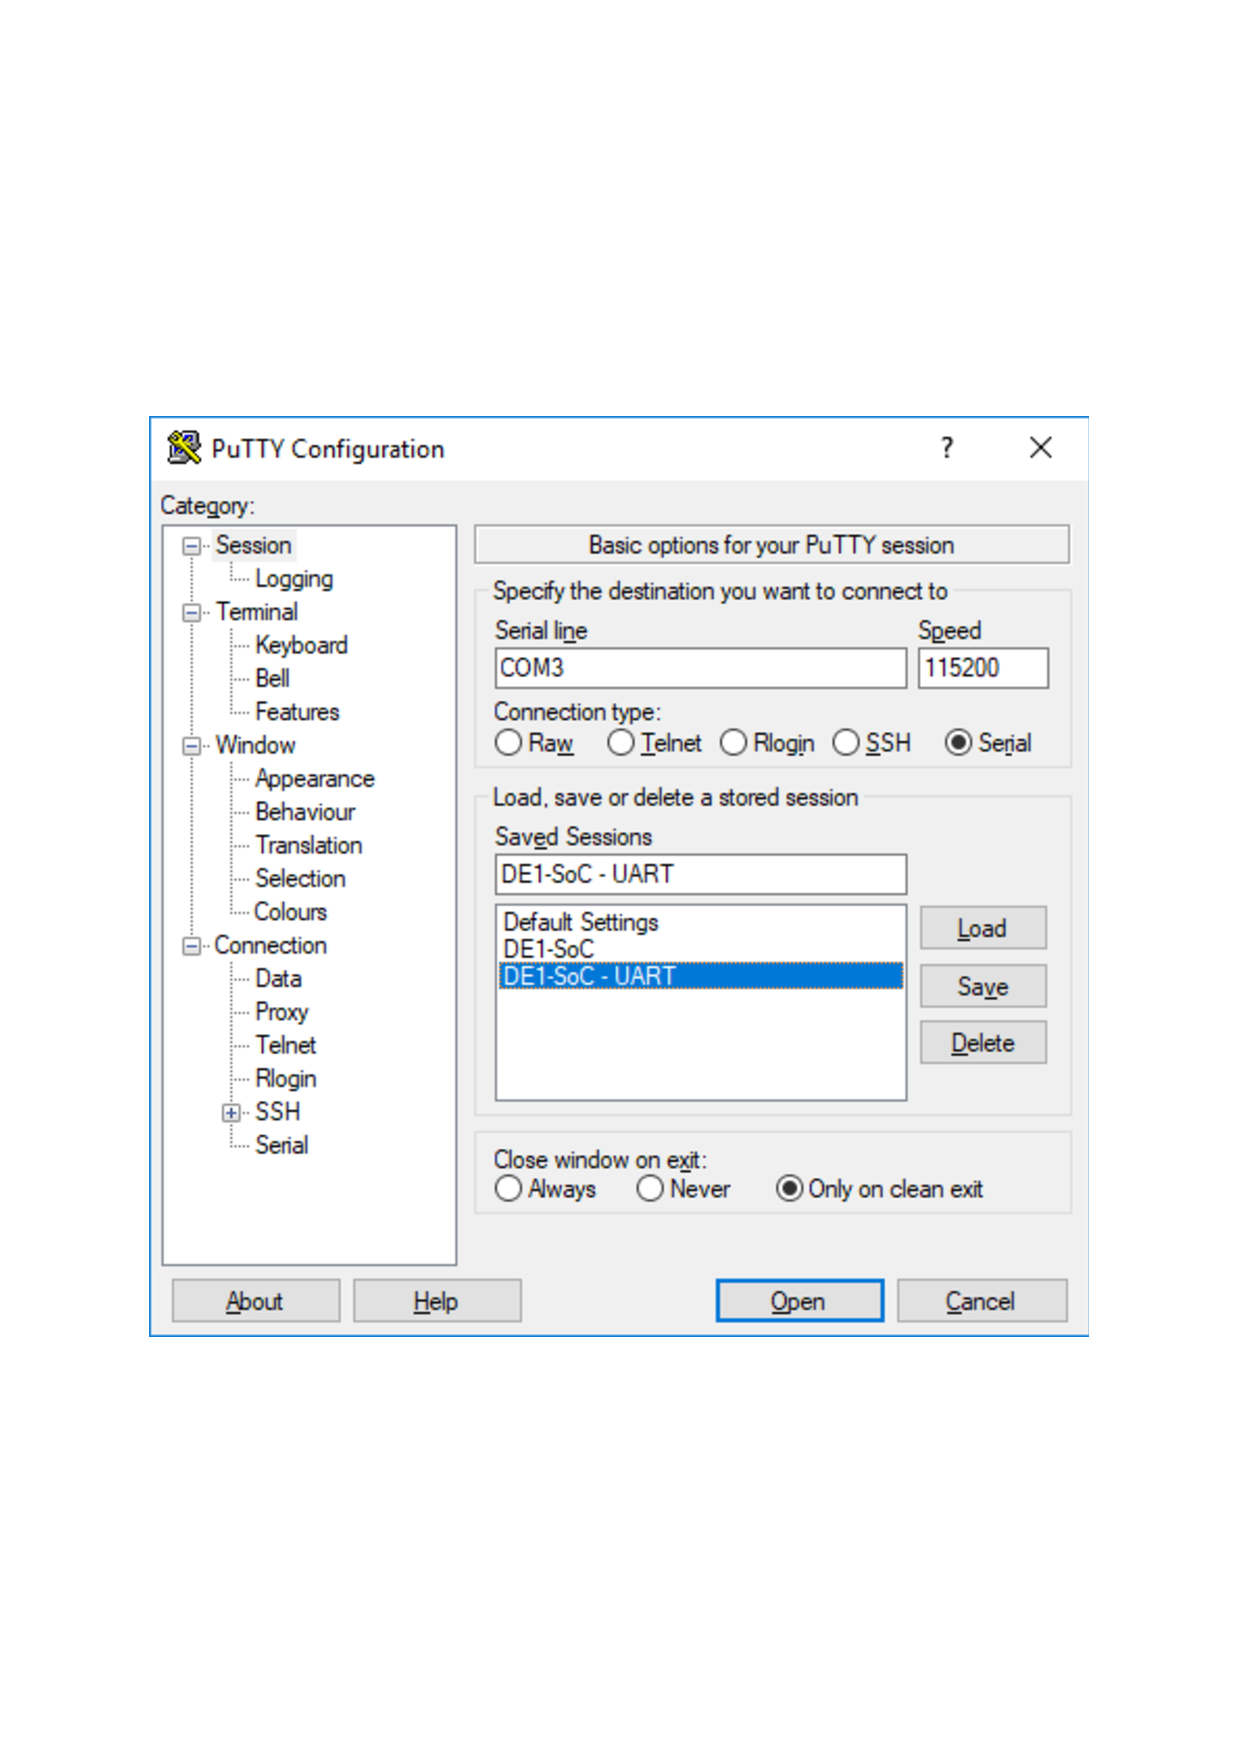
\includegraphics[width=0.9\linewidth]{images/putty_serial}
%%		\caption{Grundeinstellungen}
%%		\label{fig:putty_serial}
%%	\end{subfigure}%
%%	\begin{subfigure}{.5\textwidth}
%%		\centering
%%		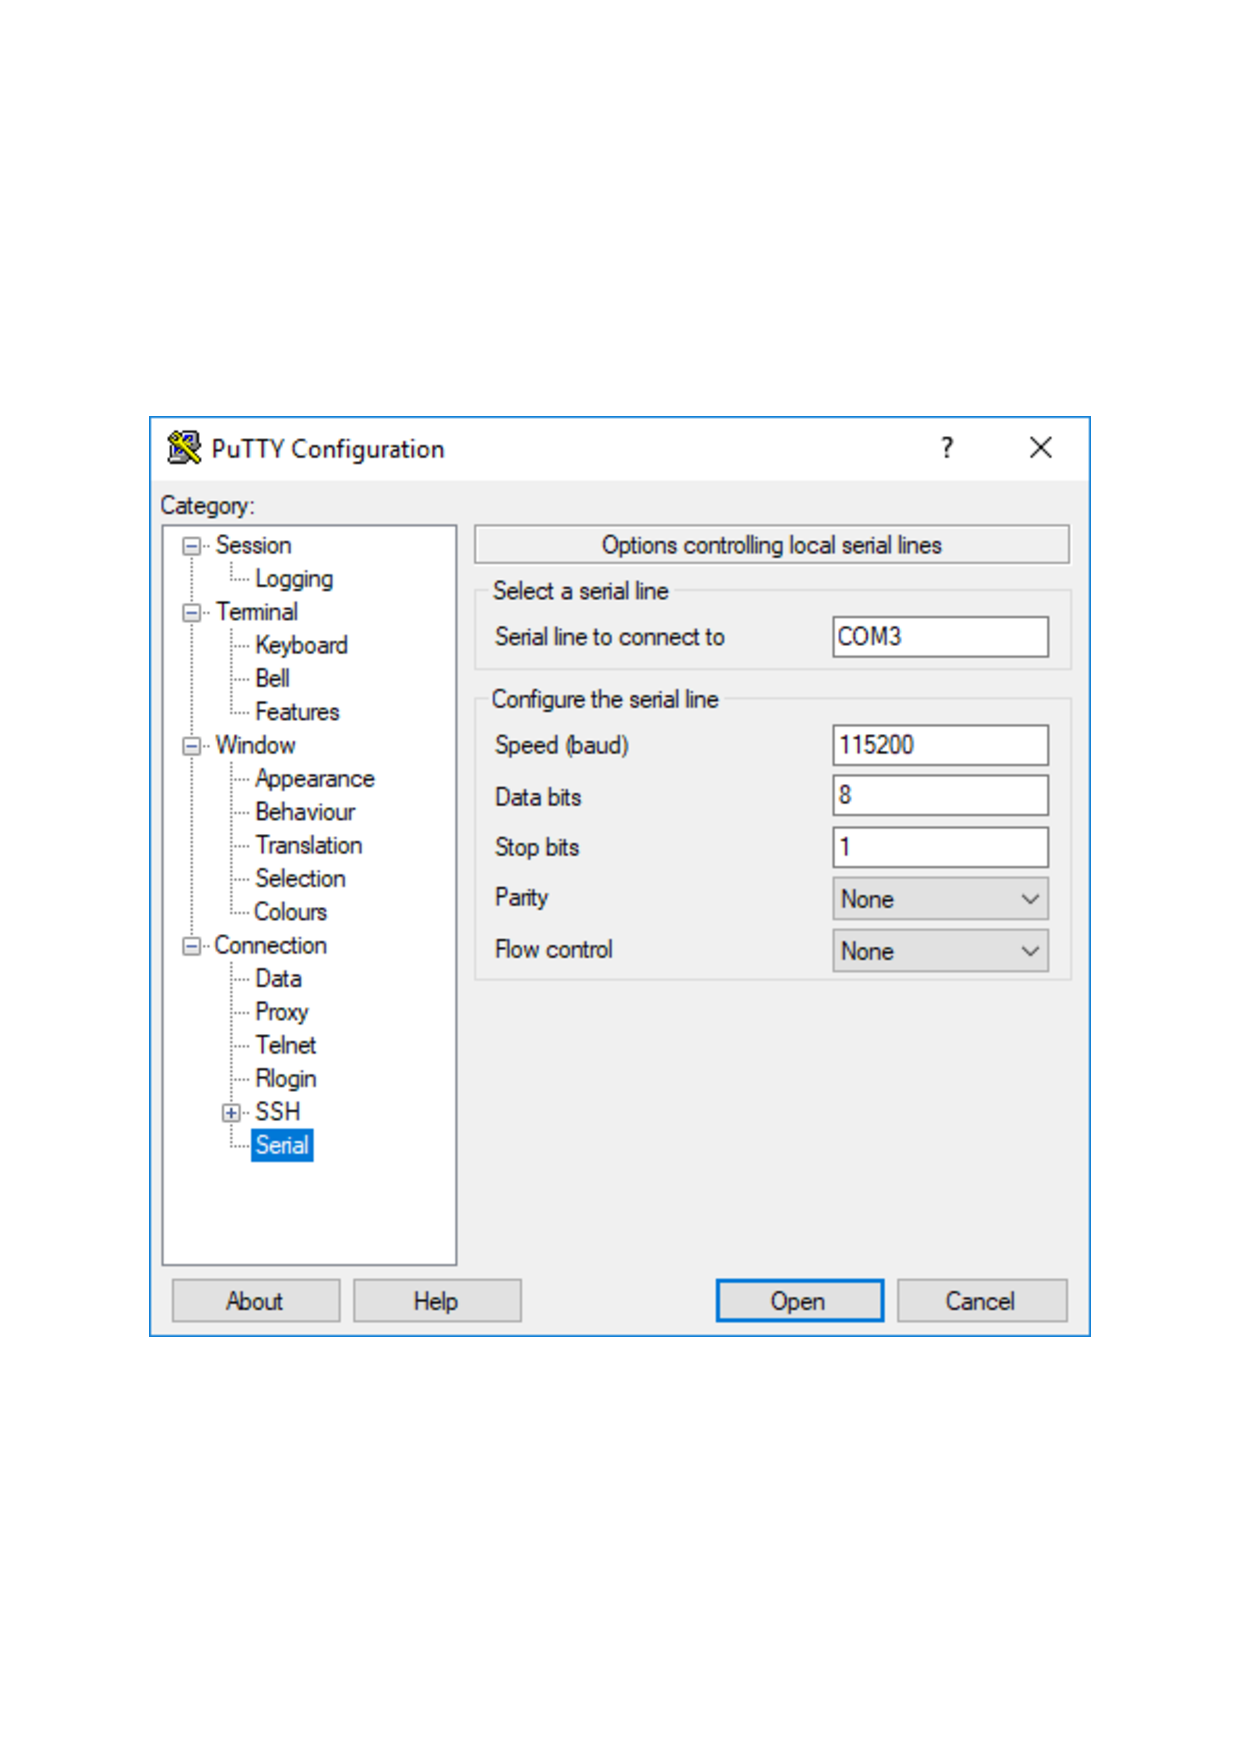
\includegraphics[width=0.9\linewidth]{images/putty_serial_params}
%%		\caption{Erweiterte Einstellungen}
%%		\label{fig:putty_serial_params}
%%	\end{subfigure}
%%	\caption{Putty-Konfiguration}
%%	\label{fig:putty}
%%\end{figure}